\documentclass[12pt,openright,twoside,a4paper,english,french,spanish]{abntex2}

\usepackage{cmap}	
\usepackage{lmodern}	
\usepackage[T1]{fontenc}	
\usepackage[utf8]{inputenc}		
\usepackage{lastpage}		
\usepackage{indentfirst}
\usepackage[table]{xcolor}	
\usepackage{graphicx}	
\usepackage{units}
\usepackage[brazilian,hyperpageref]{backref}
% \usepackage[alf]{abntex2cite}
\usepackage{bold-extra}
\usepackage{eso-pic}
%
\usepackage{tikz}
% \usepackage[]{circuitikz}
\usepackage[american,cuteinductors,smartlabels]{circuitikz}

\usepackage{lipsum}
\usepackage{listings}
\usepackage{caption}
% \usepackage[acronym]{glossaries} 
\usepackage[subentrycounter,seeautonumberlist,nonumberlist=true]{glossaries}
\usepackage[brazilian,hyperpageref]{backref}	 % Paginas com as citações na bibl
\usepackage[alf]{abntex2cite}	% Citações padrão ABNT
\usepackage{subcaption}
\usepackage{multicol}
\usepackage{multirow}
\usepackage{gensymb}
\usepackage{amsmath}

\input{fixos/comandos}
\input{fixos/novosComandos}

% Dados pessoais
\autor{}
\curso{}

% Dados do trabalho
\titulo{Posicionador de Lente}
\data{14 de maio 2014}
\palavraChaveUm{contratos}
\palavraChaveDois{ágeis}


% Dados da orientacao
\orientador{}
\coorientador{(quando houver, Titulação Acadêmica e Nome do Orientador)}

% Dados para a ficha catalográfica
\cdu{02:141:005.6}

% Dados da aprovação do trabalho
\dataDaAprovacao{01 de junho de 2013}
\membroConvidadoUm{Titulação e Nome do Professor Convidado 01}
\membroConvidadoDois{Titulação e Nome do Professor Convidado 02}

\preambulo{Trabalho de Projeto Integrador de Engenharia 2}
\local{Brasília, DF}
\instituicao{%
  Universidade de Brasília - UnB
  \par
  Faculdade UnB Gama - FGA
}
\tipotrabalho{}

\definecolor{blue}{RGB}{41,5,195}
\makeatletter
\hypersetup{
     	%pagebackref=true,
		pdftitle={\@title}, 
		pdfauthor={\@author},
    	pdfsubject={Bike-X},
	    pdfcreator={LaTeX with abnTeX2},
		pdfkeywords={Rift, }{Unity 3D, }{abntex, }{Sensores Fisiol\'ogicos, }{Ambiente Virtual}, 
		colorlinks=true,       		% false: boxed links; true: colored links
    	linkcolor=blue,          	% color of internal links
    	citecolor=blue,        		% color of links to bibliography
    	filecolor=magenta,      		% color of file links
		urlcolor=blue,
		bookmarksdepth=4
}
\makeatother
\setlength{\parindent}{1.3cm}
\setlength{\parskip}{0.2cm}  
\makeindex

\usetikzlibrary{chains}
\usetikzlibrary{shapes,arrows,shadows}
\usetikzlibrary{mindmap,trees}
\usetikzlibrary{calc,decorations.pathmorphing,patterns}
\pgfdeclaredecoration{penciline}{initial}{
    \state{initial}[width=+\pgfdecoratedinputsegmentremainingdistance,
    auto corner on length=1mm,]{
        \pgfpathcurveto%
        {% From
            \pgfqpoint{\pgfdecoratedinputsegmentremainingdistance}
                      {\pgfdecorationsegmentamplitude}
        }
        {%  Control 1
        \pgfmathrand
        \pgfpointadd{\pgfqpoint{\pgfdecoratedinputsegmentremainingdistance}{0pt}}
                    {\pgfqpoint{-\pgfdecorationsegmentaspect
                     \pgfdecoratedinputsegmentremainingdistance}%
                               {\pgfmathresult\pgfdecorationsegmentamplitude}
                    }
        }
        {%TO 
        \pgfpointadd{\pgfpointdecoratedinputsegmentlast}{\pgfpoint{1pt}{1pt}}
        }
    }
    \state{final}{}
}


% \usepackage{tikzgraphicx}

\tikzstyle{cloud} = [draw, ellipse,fill=blue!20, node distance=3cm,
    minimum height=3em]
\tikzstyle{estado} = [draw, ellipse,fill=blue!20, node distance=3cm,align=center]
\tikzstyle{teste} = [draw, diamond,fill=green!20, node distance=3cm,align=left]
%    minimum height=2em]
\tikzstyle{ciclo} =[draw, rectangle,fill=blue!20, node distance=3cm,align=center,decorate,thick,minimum height=3em]
\tikzstyle{phanton} = []   
\tikzstyle{line} = [->,right] %[draw, -latex']
\tikzstyle{retorno} = [loop above]
\tikzstyle{arrow} = [bend left,->]
\tikzset{
    %Define standard arrow tip
    >=stealth',
    %Define style for boxes
    punkt/.style={
           rectangle,
           rounded corners,
           draw=black, very thick,
           text width=6.5em,
           minimum height=2em,
           text centered},
    % Define arrow style
    pil/.style={
           ->,
           thick,
           shorten <=2pt,
           shorten >=2pt,}
}
\newglossaryentry{rift}
{
	name = Oculus Rift,
	text = \textit{Oculus Rift},
	description={Equipamento de realidade virtual para jogos eletrônicos desenvolvido pela Oculus VR e adquirido pelo \href{https://www.facebook.com/facebook}{Facebook In} em 25 de março de 2014}
}

\newglossaryentry{msp}
{
	name = MSP430,
	text = \textit{MSP430},
	description={Microcontrolador de baixa potência da Texas Instruments (TI). A versão utilizada neste projeto é a MSP430G2553, disponibilizada junto ao kit \href{http://www.ti.com/tool/msp-exp430g2}{Launchpad}}
}

\newglossaryentry{rs232}
{
	name = UART (RS232),
	text = \textit{UART},
	description={Padrão de protocolo para troca serial de dados binários entre um DTE (terminal de dados) e um DCE(comunicador de dados). Também é conhecido por \textit{EIA RS-232C} ou \textit{V.24)}}
}

\newglossaryentry{python}
{
	name = Python,
	text = \textit{Python},
	description={Python é uma linguagem de programação de alto nível , interpretada, imperativa, orientada a objetos, funcional, de tipagem dinâmica e forte. Foi lançada por Guido van Rossum em 1991\cite{python_history}. Atualmente possui um modelo de desenvolvimento comunitário, aberto e gerenciado pela organização sem fins lucrativos Python Software Foundation}
}

\newglossaryentry{puppet}
{
	name = Puppet,
	text = \textit{Puppet},
	description={Puppet é um sistema de gerenciamento de configuração que permite que que seja definido o estado da infraestrutura de TI. A ferramenta open-source é mantida pela Puppet Labs}
}

\newglossaryentry{git}
{
	name = Git,
	text = \textit{Git},
	description={É um sistema de controle e versionamento de código open-source desenvolvido por Linus Torvalds e Junio Hamano sob licença GNU GPL2. Permite o desenvolvimento distribuído, autenticação criptográfica do histórico, estratégias de mescla (merge) conectáveis dentre outras funcionalidades que agilizam a produção e garantem integração do desenvolvimento da equipe com o projeto, fazendo dele uma das gerramentas mais utilizadas atualmente para versionamento de código}
}

\newglossaryentry{cave}
{
	name = CAVE,
	text = \textit{CAVE},
	description={Caverna digital ou CAVE (Cave Automatic Virtual Environment) é um ambiente onde são projetados imagens em suas paredes (e algumas vezes chão) no intuito de explorar e interagir com objetos, pessoas virtuais e outros para ter um ambiente virtual, desta forma megulhando em um mundo virtual}
}

\newglossaryentry{chef}
{
	name = Chef,
	text = \textit{Chef},
	description={Chef é um sistema de gerenciamento de configuração que permite que que seja definido o estado da infraestrutura de TI. Usa Ruby e  domain-specific language (DSL) realizar as \textit{receitas} no sistema}
}

\newglossaryentry{ruby}
{
	name = Ruby,
	text = \textit{Ruby},
	description={Ruby é uma linguagem de programação dinâmica, refletiva, orientada à objetos de proposito de uso geral. Ela foi designada e desenvolvida nos anos 90 por Yukihiro "Matz" Matsumoto no Japan}
}


\makeglossaries

\begin{document}

\frenchspacing 
\imprimircapa
\imprimirfolhaderosto*

\begin{center}

\chapter*{Equipe}

Camila Ferreira \\
Charles Daniel \\
Gabriela Navarro \\
José Alberto \\
José Alisson \\
Julio Cezar do Nascimento \\
Lucas Konashiro \\
Luiz Fernando Gomes de Oliveira \\
Macartur Sousa \\
Priscila Pires \\
Tatiana Dias \\
Thiago Ferreira Gomes.

\vspace{3cm}

\let\clearpage\relax
\chapter*{Professores Coordenadores}

Alessandro Borges de Sousa Oliveira \\
Edson Mintsu Hung \\
Ricardo Ajax Dias Kosloski \\
Ricardo Matos Chaim  \\
Suélia de Siqueira Rodrigues Fleury Rosa \\
Thais Maia Araujo \\

\end{center}

\newpage

% \input{fixos/fichaCatalografica}
% \input{editaveis/epigrafe}
\input{fixos/indiceAutomatico}

\textual

\part{Escopo do produto}
\chapter[Problema]{Problema}

O estilo de vida do ser humano mudou drasticamente ao longo dos últimos séculos. Atividades que antes eram realizadas por pessoas passaram a ser executadas 
por máquinas, e sistemas eletrônicos, exigindo cada vez menos do corpo humano. Esta diminuição em atividades físicas tem levado as pessoas a tomar um estilo 
de vida mais sedentário, provocando um aumento nos índices de doenças crônicas como obesidade, diabetes, hipertensão e uma série de outras doenças. Desta forma, 
as organizações de saúde recomendam uma alimentação balanceada e principalmente a prática de exercícios físicos para combater os problemas causados pelo 
sedentarismo.

Dentre as diversas formas de atividade física, o ciclismo se destaca por ser uma atividade simples e agradável ao ciclista. O ciclismo permite ao praticante 
exercitar vários músculos do corpo e trabalhar a coordenação motora. Além disso, o contato com o ambiente torna esta prática mais prazerosa ao usuário. No 
entanto, existem diversos fatores que dificultam a prática desta atividade nas grandes cidades brasileiras.
A primeira das dificuldades enfrentadas por ciclistas é o acesso a espaços apropriados para a prática do ciclismo. A ausência de ciclovias obriga ao ciclistas 
a utilizar as ruas e a dividir espaço com motoristas, que geralmente não aceitam dividir o espaço pelo fato dos ciclistas trafegarem em velocidades menores que 
a dos carros, podendo causar acidentes. Mesmo quando há ciclovias, os ciclistas tem de enfrentar as avenidas urbanas para chegar ao local, novamente interagindo 
com motoristas.

Outros fatores que tornam a prática do ciclismo mais difícil envolvem questões relacionadas a falta de estrutura urbana. Muitas cidades brasileiras não são 
planejadas para o ciclismo, mesmo como forma de locomoção, pois quando há ciclovias, elas são geralmente descontínuas. 

Em Pelotas, Rio Grande do Sul, Brasil, \cite{barros2003}, comparando informações de boletins de ocorrência e atendimentos no pronto-socorro durante dois anos, encontraram 33,0\% de sub-registros relativos aos acidentes com lesão corporal envolvendo ciclistas.

Buracos e falta de recapeamento nas ciclovias também podem acarretar em acidentes e causar lesões aos ciclistas. Os ciclistas mais regulares afirmam também que a falta de bicicletários os obrigam a improvisar formas de fixar seu veículo. Outro fator que contribui para as dificuldades enfrentadas por ciclistas é a falta de segurança e de estrutura em espaços públicos, onde a falta de iluminação ou mesmo as abordagens de assaltantes tornam a prática mais arriscada.

Para as pessoas que não praticam atividades físicas, a principal justificativa é a falta de tempo com relação a suas atividades diárias. Em especial para o 
ciclismo, de fato, é necessário um gasto de tempo até a chegada em uma área apropriada para uma circulação mais tranquila de bicicletas. Como alternativa, as 
bicicletas ergométricas que em sua maioria estão presentes em academias são um incentivo a prática do ciclismo e devido a sua estrutura mecânica, tendem a ser 
mais confortáveis para o praticante.
Outra característica destas bicicletas é que pelo fato de serem fixas, oferecem menos riscos de lesões causadas por quedas. Além disso, o stress causado pelo 
trânsito em avenidas movimentadas não existe para este caso. Apesar de permitir simular os movimentos da pedalada de uma bicicleta comum, a bicicleta ergométrica 
tem a desvantagem de não oferecer estímulo do ambiente ao usuário. Com isso, exercitar-se em uma bicicleta ergométrica se torna uma atividade monótona ao 
praticante.



\chapter*[Proposta]{Proposta}
\addcontentsline{toc}{chapter}{Proposta}

\chapter*[Projeto]{Projeto}
\addcontentsline{toc}{chapter}{Projeto}

\chapter[Requisitos do produto]{Requisitos do produto}

A fim de deixar claro quais os limites do projeto, foram estabelecidos os requisitos funcionais e não funcionais do produto. São eles:
\begin{itemize}
	\item Requisitos Funcionais do produto
		\begin{itemize}
		\item permitir ao usuário admirar a paisagem virtual assim como a real
		\item permitir ao usuário acelerar e desacelerar a bicicleta virtual
		\item permitir ao usuário fazer curvas para direita e para a esquerda
		\item permitir ao usuário trocar as marchas da bicicleta virtual
		\item permitir ao usuário recarregar a bateria de seu dispositivo móvel
		\item apresentar ao usuário a velocidade virtual, distância percorrida, número de batimentos cardíacos por minuto, quantidade de calorias gastas, tempo gasto e a energia elétrica
		\end{itemize}
	\item Requisitos não funcionais do produto:
		\begin{itemize}
		\item dar a sensação ao usuário de pedalar em trechos com subida
		\item dar ao usuário sensação de conforto(ergonomia) ao pedalar a bicicleta
		\item dar ao usuário sensação de conforto durante a imersão virtual
		\item converter energia mecânica em elétrica para retroalimentação da bicicleta
		\end{itemize}
\end{itemize}

\chapter[Análise do Impacto Social e Ecônomico do Posicionador de Lente]{Análise do Impacto Social e Ecônomico do Posicionador de Lente}

O produto que está sendo desenvolvido, Posicionador de Lente, é um produto inexistente atualmente no mercado. Com isso, a sua inserção no mercado ocasionará impactos de natureza
social e econômica. Nas seções a seguir será apresentado e discutido cada um deles. É importante relembrar os dois problemas que esse produto procura resolver: limpeza inadequada e dificuldade de utilização. A limpeza inadequada está fortemente relacionada ao impacto social que o produto irá gerar,  pois reduzirá eventuais doenças causadas pela limpeza inadequada, enquanto a dificuldade de utilização está relacionada tanto ao impacto social quanto ao impacto econômico, pois as pessoas irão adquirir o produto porque não conseguem utilizar lentes de contato sem ele, seja qual for a dificuldade.

\section[Impacto Social]{Impacto Social}

\subsection[Redução de doenças causadas pela limpeza inadequada]{Redução de doenças causadas pela limpeza inadequada}

A correta manutenção das lentes de contato é fundamental para se obter
sucesso e manter a continuidade de seu uso. É grande o número de
pacientes que abandonam o uso de suas lentes por problemas que poderiam
ser solucionados com tratamentos relativamente simples ou com uma
orientação mais adequada. O mau uso das lentes, associado à má adaptação,
contaminação, doenças oculares prévias e fatores ambientais, podem
aumentar o número de infecções corneanas através da proliferação de
microorganismos. 

A importância da manutenção das lentes de contato (LC) é fundamental
para se obter sucesso e manter a continuidade de seu uso, já que as
complicações oculares devido à falta de obediência dos usuários em relação
à manutenção e ao período de troca, em conjunto com a ausência de
motivação estão entre as principais causas da desistência do paciente \cite{coral}.

É grande o número de pacientes que abandonam o uso de suas lentes
por causa de problemas que poderiam ser solucionados com tratamentos
relativamente simples \cite{vieira}. Um fator decisivo para que algumas
pessoas desistam de usar suas lentes é a manutenção inadequada ou o uso
incorreto. 

O mau uso das lentes, associado à má adaptação, contaminação, doenças
oculares prévias e fatores ambientais, podem aumentar o número de
infecções corneanas através da proliferação de microorganismos como
bactérias, fungos, parasitas, vírus, uma vez que o próprio uso da lente
altera o mecanismo de defesa do olho \cite{robert}.

As soluções multiuso vieram para facilitar o paciente no
cuidado das LC, uma vez que limpeza, enxágüe e desinfecção
são feitos com o mesmo produto. Suas macromoléculas reduzem
a penetração do desinfetante na córnea, limitando seu
acúmulo na matriz da lente.

Ao contrário do que ocorria há alguns anos, quando os
usuários tinham que limpar suas lentes com inúmeros produtos
diferentes ou até fervê-las, a manutenção tornou-se, atualmente,
mais simples e prática, o que pode fazer o paciente
aderir mais facilmente aos procedimentos \cite{rakow}.

Toda lente, independente de ser rígida ou gelatinosa,
descartável ou convencional, deve, a princípio, passar por
um processo de manutenção que inclua limpeza diária, desinfecção
e retirada dos depósitos de proteínas. Os procedimentos comuns para limpeza de lente são: limpeza do estojo, higienização das mãos, limpeza das lentes, enxague e desinfecção.

A manutenção correta das lentes é essencial na prevenção
de complicações infecciosas, tóxicas e alérgicas, bem como
para o conforto de seu uso. Como já frisamos anteriormente, é
grande o número de pacientes que abandonam as lentes por
complicações causadas por falta de cuidados ou produtos
inapropriados \cite{moreira}.

Assim, um produto como o Posicionador de Lente realizaria de forma automática os procedimentos comuns de limpeza de lente, fazendo com que o usuário interfira minimamente sobre o processo, sendo necessária uma intervenção apenas mensal para manutenção do aparelho. Com isso, o número de desistentes e de possíveis doenças causadas pela limpeza inadequada reduziria.

Outro fato importante é que muitas pessoas ao desistirem de utilizar lentes de contato, deixam de lado também os óculos de grau ou um acompanhamento oftalmológico adequado, fazendo com que as doenças oftalmológicas permaneçam ou se agravam em médio ou longo prazo. 

\subsection[Promoção à Saúde e Qualidade de Vida - Projeto Olhar Brasil]{Promoção à Saúde e Qualidade de Vida - Projeto Olhar Brasil}

São conhecidos os altos percentuais de problemas oftalmológicos que afetam a população 
brasileira e a desigual distribuição dos recursos humanos e financeiros para a sua abordagem. Os 
problemas visuais respondem por grande parcela de evasão e repetência escolar, pelo desajuste 
individual no trabalho, por grandes limitações na qualidade de vida, mesmo quando não se trata 
ainda de cegueira \cite{olhar}.

O SUS dispõe de 2.374 unidades de saúde que realizam consulta oftalmológica. No ano 
de 2005, foram realizadas 7.815.134 consultas oftalmológicas e fornecidos 91.390 óculos. O 
número de oftalmologistas, no Sistema Único de Saúde, totaliza 5.701 profissionais, sendo que a 
maior concentração de médicos oftalmologistas e de unidades de saúde está nas regiões sul e 
sudeste
, com 57\% do total de serviços; 32\% nas regiões norte e nordeste e 11\% na região 
centro-oeste \cite{olhar}.

Evidencia-se a necessidade de realização de novas ações que atendam com maior 
resolutividade à crescente demanda ampliando o acesso da população aos serviços de 
oftalmologia. Com isso, foi criado e implatado o Projeto Olhar Brasil, cujos objetivos são:
\begin{enumerate}
\item Identificar problemas visuais, relacionados a refração, em alunos matriculados na rede 
pública de ensino fundamental (1ª a 8ª série), no programa “Brasil Alfabetizado” do MEC 
e população acima de 60 anos de idade; 
\item  Prestar assistência oftalmológica com fornecimento de óculos nos casos de erro de 
refração; 
\item Otimizar a atuação dos serviços especializados em oftalmologia, ampliando o acesso à
consulta, no âmbito do SUS; 
\item Garantir a referência para serviços especializados nos casos que necessitarem de 
intervenções de Média e Alta Complexidade em Oftalmologia; 
\item Criar um banco de dados com informações do desenvolvimento do Projeto; 
\item Propiciar condições de saúde ocular favorável ao aprendizado do público alvo 
melhorando o rendimento escolar dos estudantes do ensino público fundamental, jovens e 
adultos do programa Brasil Alfabetizado de forma a reduzir as taxas de evasão e 
repetência; 
 \end{enumerate}

Esse projeto atinge cerca de 2 milhões de pessoas. Se uma parceria fosse realizada com o produto Posicionador de Lente o impacto social seria grande. Pois assim como o uso de óculos de grau aumentam a qualidade de vida dessas pessoas, o uso adequado de lentes de contatos iria aumentar ainda mais a auto estima das pessoas: muitas delas não aderem de forma completa ao Projeto Olhar Brasil por não desejarem usar óculos de grau ou os utilizam eventualmente.


\section[Impacto Econômico]{Impacto Econômico}

A dificuldade de utilização de lentes de contato interfere diretamente na venda das mesma. Com a inserção do Posicionador de Lente no mercado, a projeção de vendas de lentes de contato de diversos tipos será crescente. Por exemplo, o público feminino, que é um dos que possuem dificuldade de utilização devido ao comprimento das unhas, seria um grande consumidor tanto do Posicionador de Lente quanto das lentes de contato. Dos dados mais estáveis que foram capturados cerca de 67\% das lentes foram prescritas para mulheres em 2012.
\part{Planejamento}
\chapter[Divisões]{Divisões}
% \addcontentsline{toc}{chapter}{Divisões}

\section{Equipe}
\begin{itemize}
	\item Automotiva
		\begin{itemize}
			\item Tatiana Dias
		\end{itemize}
	\item Eletrônica
		\begin{itemize}
			\item José Alison
			\item José Alberto Alves de Andrade
		\end{itemize}
	\item Energia
		\begin{itemize}
			\item Priscila Pires
			\item Thiago Gomes
			\item Júlio César do Nascimento
		\end{itemize}
	\item Software
		\begin{itemize}
			\item \textbf{Charles Daniel* (Gestor)}
			\item Camila Fereira
			\item Gabriela Matias
			\item Lucas Kanashiro
			\item Luiz Fernando Gomes de Oliveira
			\item Macártur Souza
		\end{itemize}
\end{itemize}

\section{Divisão das tarefas}
Para a construção do produto, a equipe designou a divisão de tarefas por áreas da seguinte forma:

\begin{itemize}
	\item Automotiva
		\begin{itemize}
		\item Ergonomia
		\item Análise estrutural
		\end{itemize}
	\item Eletrônica
		\begin{itemize}
		\item Construção dos circuitos biológicos
		\item Bibliotecas para uso de comunicação e coleta de dados no microcontrolador
		\end{itemize}
	\item Energia
		\begin{itemize}
		\item Armazenamento de energia
		\item Dimensionamento dos dispositivos responsáveis conversão eletromecânica de energia
		\item Dimensionamento do circuito de distribuição da energia e do circuito de proteção da malha
		\item Verificação da eficiência energética
		\end{itemize}
	\item Software
		\begin{itemize}
		\item Construção do Ambiente Virtual
		\item Interface de comunicação com sensores
		\item Interface de comunicação com o motor de freio
		\end{itemize}
\end{itemize}

\chapter[Materiais]{Materiais}

Para a execução do presente projeto foram levantados os materiais que serão requisitados para a correta condução deste trabalho. Assim, são informados a seguir 
os materiais necessários, bem como o papel executado por cada material.

\section{Sistema Mecânico/Suporte de apoio}

\begin{itemize}
\item Bicicleta – será o meio pelo qual o usuário do produto realizará atividade física, e a partir dessa atividade, serão gerados dados que servirão de 
  entrada para os sensores. Também será a partir dessa atividade que ocorrerá o acionamento mecânico do gerador.
\item Cavalete – servirá de apoio para a roda traseira da bicicleta, de maneira que esta não entre em contato com o solo.
\end{itemize}

\section{Circuito Elétrico}

Em relação ao circuito elétrico que será responsável para a conversão eletromecânica de energia, distribuição dessa entre os diversos elementos da malha, 
bem como os dispositivos de proteção do mesmo, serão necessários os seguintes materiais:

\begin{itemize}
\item Gerador – será o elemento do circuito que irá realizar a conversão eletromecânica da energia oriunda do sistema escopo deste projeto. Para isso, será 
  utilizado um gerador que utiliza o princípio da indução eletromagnética; especificamente, utilizar-se-á um alternador automotivo.
\item Condutores – terão a responsabilidade de permitir o trânsito de corrente elétrica entre os diversos dispositivos do circuito. Convém informar que as 
  bitolas dos condutores serão dimensionadas visando atender as características elétricas das cargas que serão alimentadas.
\item Dispositivos de proteção – responderão pela segurança do circuito, isto é, cuidarão para que o circuito responda de maneira adequada quando submetido a 
  possíveis distúrbios de ordem elétrica. Assim, permitirão segurança pessoal, integridade dos dispositivos do circuito, bem como isolar o sistema em caso de 
  falta. Para o nosso projeto, propõe-se o uso de fusíveis.
\item Direcionadores de corrente – serão utilizados com o intuito de garantir a correta polarização do circuito em comento. Nesse sentido, serão selecionados 
  diodos que atendam aos requisitos do nosso circuito.
\item Bateria – será o elemento do circuito que armazenará parcela da energia eletromecânica convertida. Desse modo, em caso de falta, ou após a paralisação 
  de funcionamento do gerador, a bateria será responsável pela continuidade da alimentação elétrica das cargas do circuito, garantido certo nível de confiança 
  de fornecimento de energia para as cargas existentes.
\item Multímetro – responsável pela medição das grandezas de ordem elétrica do circuito, tais como tensão e corrente elétrica.
\item Inversor de tensão – será o dispositivo do circuito responsável pela mudança de corrente contínua para corrente alternada.
\item Regulador de tensão – este dispositivo será utilizado para controlar as possíveis flutuações de tensão que poderão existir no circuito, garantindo assim, 
  a correta potência para cada carga.
\item Interruptor – terá a responsabilidade de seccionar temporariamente uma parte do circuito, e também desligá-lo, quando não estiver sendo utilizado. 
\end{itemize}

\section{Cargas}

Os materiais relacionados às cargas que serão conectadas ao circuito elétrico pertinente ao projeto em discussão são indicados a seguir:

\begin{itemize}
\item Dispositivo móvel – uma vez que ocorrerá conversão eletromecânica de energia, parcela dessa energia será disponibilizada para alimentar algum
  dispositivo móvel de interesse do usuário.
\item Sensores – serão alimentados eletricamente sensores que detectarão dados de interesse para o projeto, sendo esses dados repassados ao usuário.
\item Potenciômetro - para detectar virada do guidão.
\item Notebook;
\item Oculus Rift;
\item MSP430 - microcontrolador responsável por coletar os dados dos sensores e transmiti-los para o computador.
\end{itemize}

\section{Software}

Unity 4 – será responsável pela modelagem do ambiente virtual que será exibido ao usuário através do \textit{Oculus Rift}.


% \section{MSP430} % (fold)
\label{sec:msp430}

É um microcontrolador RISC de 16 bits criado pela Texas Instrumets para aplicações de baixo consumo de energia.

% section msp430 (end)

% \section{Unity 3D} % (fold)
\label{sec:unity_3d}

\subsection{O Unity }
\label{sub:o_unity}
	A unidade é um IDE de desenvolvimento de jogos com um potente mecanismo de renderização e totalmente integrado com um conjunto de ferramentas que permitem criação de conteúdos interativos em varias plataformas e em  3d ou 2d.Além disso é possivel gerar builds para de 16 plataformas  como o linux , android ,windows e iOS com um alto nivel de qualidade pois é possível utilizar recursos prontos da Assert Store e de comunidades de compartilhamento de conhecimentos. 
	Para esse projeto foi escolhido o Unity pois  além dos benefícios citados acima com ele é possível que o desenvolvimento seja mais agil, em menos tempo e com umcusto menor e com uma qualidade razoável. 

\subsection{Workflow} % (fold)
\label{sub:workflow}
	Com o intuito de simplificar o processo de criação e produção de software, o Unity oferece um ambiente de trabalho com diversas ferramentas integradas para o desenvolvimento para a possibilitar a criação de mundos complexos com bloco de construção de cenas rapidamente escaláveis, implementar fluxos de controle utilizando linguagens altamente utilizadas no mercado como C\# e Java Script, com uma perfomace de tempo de compilação. Além disso durante o processo de criação é possível economizar tempo utilizando elementos prontos, salas e forúm de bate papo para distribuição de conhecimentos e resolução de problemas e dúvidas.

\begin{figure}[h]
  \centering
  \includegraphics[width=0.8\textwidth]
      {figuras/bike.png}
  \caption{Edição de objeto no Unity}
  \label{coordenadas-rift}
\end{figure}

\subsection{Modelagem de Elementos} % (fold)
\label{sub:modelagem}
	Para a utilização de elementos no Unity é necessario a criação de objetos 3d, para isso pode ser utilizado qualquer um das IDE mais utilizadas do mercado tais como Maya , 3DMax, Blender ,Cinema4D, Modo, Lightwave, Cheetah3D, entre outros. A manipulação e ajustes de objetos em 3D está sendo realizada através da utilização da ferramenta blender  que é uma plataforma livre de alto desempenho que permite além da modelagem para a criação de objetos 3D e contém ferramentas para animações, criação de jogos, construção de foto realismo, simulações de fluidos, edição de vídeos,entre outros.Depois de feito os ajustes nos modelos o Blender possui suporte para exportar objetos nos formatos de arquivo: 3DS,DXF,FBX,OBJ,LWO,SVG,STL entre outros.

\begin{figure}[h]
  \centering
  \includegraphics[width=0.8\textwidth]
      {figuras/blender.png}
  \caption{Renderização de \textit{Bick Buck Bunny} sendo feita no Blender}
  \label{coordenadas-rift}
\end{figure}

\subsection{SDK OculusVR}
\label{sub:sdk_ovr}
      Nos primeiros passos para a integração do Oculus Rift com o Unity foi necessário a utilização de uma SDK\footnote{ SDK encontrada em \url{https://developer.oculusvr.com/?action=dl&v=8 }} do próprio Oculus Rift ,que atualmente possui as versões 0.2, 0.3 e 0.4, que permite extrair dados do oculus e manipulos utilizando C++. No entanto como o Unity possui suporte para o plugin do Oculus Rift, que são scripts oriundos da SDK que ao invés de ser implementada em C++ é implementada em C\#, foi adotado o mesmo para auxiliar no controle do ambiente virtual no Unity.

\subsection{Criação de Scripts}
\label{sub:criacao_de_scripts}







\section{Oculus Rift} % (fold)
\label{sec:oculus_rift}

O \textit{Oculus Rift}\cite{oculusVR} é um produto desenvolvido pela Oculus VR\textsuperscript{\textregistered} que foi fundada por Palmer Luckey, um entusiasta em realidade virtual e \textit{nerd} de hardware. A companhia lançou uma campanha no \textit{Kickstarter}\cite{kickstarter}, uma plataforma que permite inventores encontrar patrocinadores, para ajudar a levantar fundos para seu primeiro produto, o \textit{Oculus Rift}, um óculos de imersão virtual bastante inovador para jogos. Com o suporte de gigantes produtoras de jogos eletrônicos como a Valve, Epic Games e Unity, o \textit{Kickstarter} foi o maior sucesso, levantando mais de US\$2,4 milhões em fundos. O time atualmente trabalha fortemente na comercialização do \textit{Oculus Rift}, que promete revolucionar a maneira que as pessoas interagem com conteúdos. 

\subsection{Especificações de Hardware}
O \textit{Oculus Rift} é produzido somente em versões de desenvolvimento, não se sabe ao certo quais serão as especificações de hardware para o produto comercializável. A listagem a seguir apresenta as características de hardware do \textit{Oculus Rift DK1} (primeira versão de desenvolvimento):
\begin{itemize}
	\item Especificações da tela:
		\begin{itemize}
			\item Área visível de 7 polegadas
			\item Resolução total de 1280x800, 640x800 para cada olho
			\item Distancia fixa de 64mm entre os centros das lentes
			\item LCD com frequência de 60Hz
			\item HDMI 1.3+
		\end{itemize}
	\item Especificações dos sensores:
		\begin{itemize}
			\item Ate 1000Hz de taxa de amostragem
			\item Giroscópio de três eixos, para sensorear velocidade angular
			\item Magnetômetro de três eixos, para sensoriais campos magnéticos
			\item Acelerômetro de três eixos, para sensorear a aceleração, incluindo a gravitacional
		\end{itemize}
	\item Conexoes:
		\begin{itemize}
			\item USB 2.0 para transmissão de dados dos sensores
			\item HDMI para transmissão de imagens
			\item Fonte de energia para alimentação do óculos
		\end{itemize}
\end{itemize}

%exemplo de uso do glossário
%O \gls{rift}  é um equipamento de realidade virtual para jogos eletrônicos.

% \input{editaveis/automotiva}
% \input{editaveis/energia}
\chapter*[Interações]{Interações Entre as Áreas}
\addcontentsline{toc}{chapter}{Interações}

O projeto Bike-x contará com a interação das engenharias de Software, Energia, Automotiva e Eletrônica. Esta seção visa identificar e exemplificar cada uma das interações. 

As engenharias de software e eletrônica vão se unir na área de coletar informações do sistema de forma geral e gerar respostas a partir das mesmas. A área de engenharia eletrônica será responsável em fazer que os microcontroladores leiam dados de diversos sensores, tais como: oximetria e potenciômetro para definir a direção do guidão.  A engenharia de software irá coletar essas informações e gerará respostas para interagir com o usuário, informando os valores ou agindo no sistema.

As engenharias de energia e software irão interagir utilizando a eletrônica como intermediária. Haverá um sensor que medirá a quantidade de energia gerada pelo usuário e essa informação será tratada pela engenharia de software para que o usuário tenha acesso a essa informação de forma de pop up no ambiente virtual.

As engenharias de automotiva e software também irão interagir utilizando a eletrônica como mediadora. Uma das interações com o sistema será que quando houver uma subida no ambiente virtual, o software irá gerar uma alteração no sistema. Quando isso houver, a bicicleta irá ser freada pelo (pegar nome do motor que freia a bicicleta).

O sensor que mede a quantidade de energia produzida será responsável pela interação das engenharias de energia e eletrônica. Com esse sensor será possível mostrar ao usuário quantos (pegar unidade de medida) de energia ele conseguiu produzir. 

Durante uma subida no ambiente virtual, o sistema deverá freiar a bicicleta para que o usuário sinta resistência ao pedalar e tenha a impressão de maior dificuldade de pedalar e que realmente pense que esteja em uma subida. Essa será a interação de engenharia eletrônica e automotiva.

Por fim, a interação das engenharias de energia e automotiva será feita pela adaptação do alternador no sistema para a geração de energia. Esse alternador será adaptado no rolo que usaremos para que o usuário possa pedalar sem se mover e com esse movimento a energia será gerada para alimentar o sistema.


\chapter[Organização do Trabalho]{Organização do Trabalho}

Para a realização do projeto de forma eficiente e organizada, dividiu-se inicialmente o grupo em quatro subgrupos, cada um destes representando uma das 
engenharias (automotiva, eletrônica, energia e software), e cada subgrupo tendo um representante. No decorrer do projeto, de acordo com as demandas, os 
integrantes dos subgrupos deverão ser permutados. 

Haverá em média cinco reuniões semanais com duração de duas horas entre os integrantes do projeto, sendo três delas durante as aulas e duas extra classe.
O grupo decidiu utilizar uma abordagem ágil de gerenciamento de projeto, tendo em vista que a mesma funciona bem com times pequenos, concentrando ao máximo
o esforço do time em agregar valor ao produto proposto. Esse tipo de abordagem irá favorecer a integração do grupo de trabalho, objetivo principal da disciplina.

As decisões importantes a serem tomadas, como a definição do tema do projeto, as divisões e os principais resultados esperados, são feitas por 
todos os componentes do grupo durante os horários de reunião. Além das tomadas de decisões, as reuniões serão aproveitadas para cada subgrupo se reunir, 
trabalhar em sua determinada área, apresentar e discutir seus resultados obtidos para os demais subgrupos e, quando necessário, apresentar suas principais 
dificuldades e questionamentos para os professores da disciplina. Essas horas também serão úteis para que as tarefas em que é necessário mais de um subgrupo 
para sua realização sejam cumpridas através da reunião entre os mesmos para coletar as informações necessárias e discutir os melhores métodos e soluções para 
essas tarefas.

Foi estimada uma média de quatro horas semanais de trabalho além das seis horas de aula para cada componente do grupo, a fim de concluir as tarefas e metas 
propostas para cada um desses. Essas horas são utilizadas em sua maioria para pesquisas, testes, simulações e atualizações do relatório. 

Segundo \cite{XPxRUP2006}, metodologias ágeis também dividem o desenvolvimento do software em iterações, buscando redução de riscos ao projeto. Ao final de cada iteração, uma versão (\textit{release}) funcional do produto, embora restrita em funcionalidades, é liberada ao cliente. As metodologias ágeis destacam aspectos humanos no desenvolvimento do projeto, promovendo interação na equipe de desenvolvimento e o relacionamento de cooperação com o cliente. Comunicação face-a-face é preferida à documentação compreensiva.

Com o objetivo de aperfeiçoar a integração entre os componentes dos grupos e para que cada um possa acompanhar o andamento do projeto são utilizadas algumas 
ferramentas e práticas ágeis, como \textit{software} de gerenciamento de projeto e \textit{daily meetings}. Assim, de modo que cada componente e/ou subgrupo 
possa acompanhar o que os outros estão fazendo no projeto está sendo utilizado: a ferramenta livre \href{http://lappis.unb.br/redm}{Redmine}, onde são apresentadas as tarefas, seus andamentos e o 
responsável por cada uma delas em um quadro \textit{kanban}; e os encontros diários, onde todos dizem o que foi feito, o que está sendo feito, as dificuldades
e o que será feito, possibilitando com que os principais problemas e dificuldades sejam detectados e solucionados por todos em conjunto. Para o agrupamento 
dos dados e pesquisas coletadas, além dos testes e resultados gerados e atualizações do relatório, é utilizada a ferramenta Google Docs.

Está sendo utilizada a ferramenta Git para realizar o controle de versão tanto dos códigos fonte gerados quanto dos documentos e apresentações, e como Source
Forge está sendo utilizado o GitHub. Sendo o Git uma ferramenta livre e o GitHub gratuito.

Com essa maneira de organizar o tempo, as tarefas e as equipes, espera-se que o andamento do projeto seja satisfatório, integrando as engenharias através do 
trabalho entre os subgrupos de maneira eficiente. Além disso, objetiva-se o melhor aproveitamento possível das horas disponíveis e determinadas para a realização 
do projeto por todos os componentes, de modo que a divisão de trabalho seja equilibrada ao longo do projeto, o que pode ser observado e analisado através das 
ferramentas utilizadas para o controle e divisão de tarefas.


\chapter[Cronograma]{Cronograma}
\addcontentsline{toc}{chapter}{Cronograma}

Para gerenciamento do projeto estamos utilizando a ferramenta Redmine, com esta ferramenta é possível fazer o gerenciamento do projeto no contexto ágil que é o que está sendo utilizado no Projeto.

\begin{figure}[h]
  \centering
  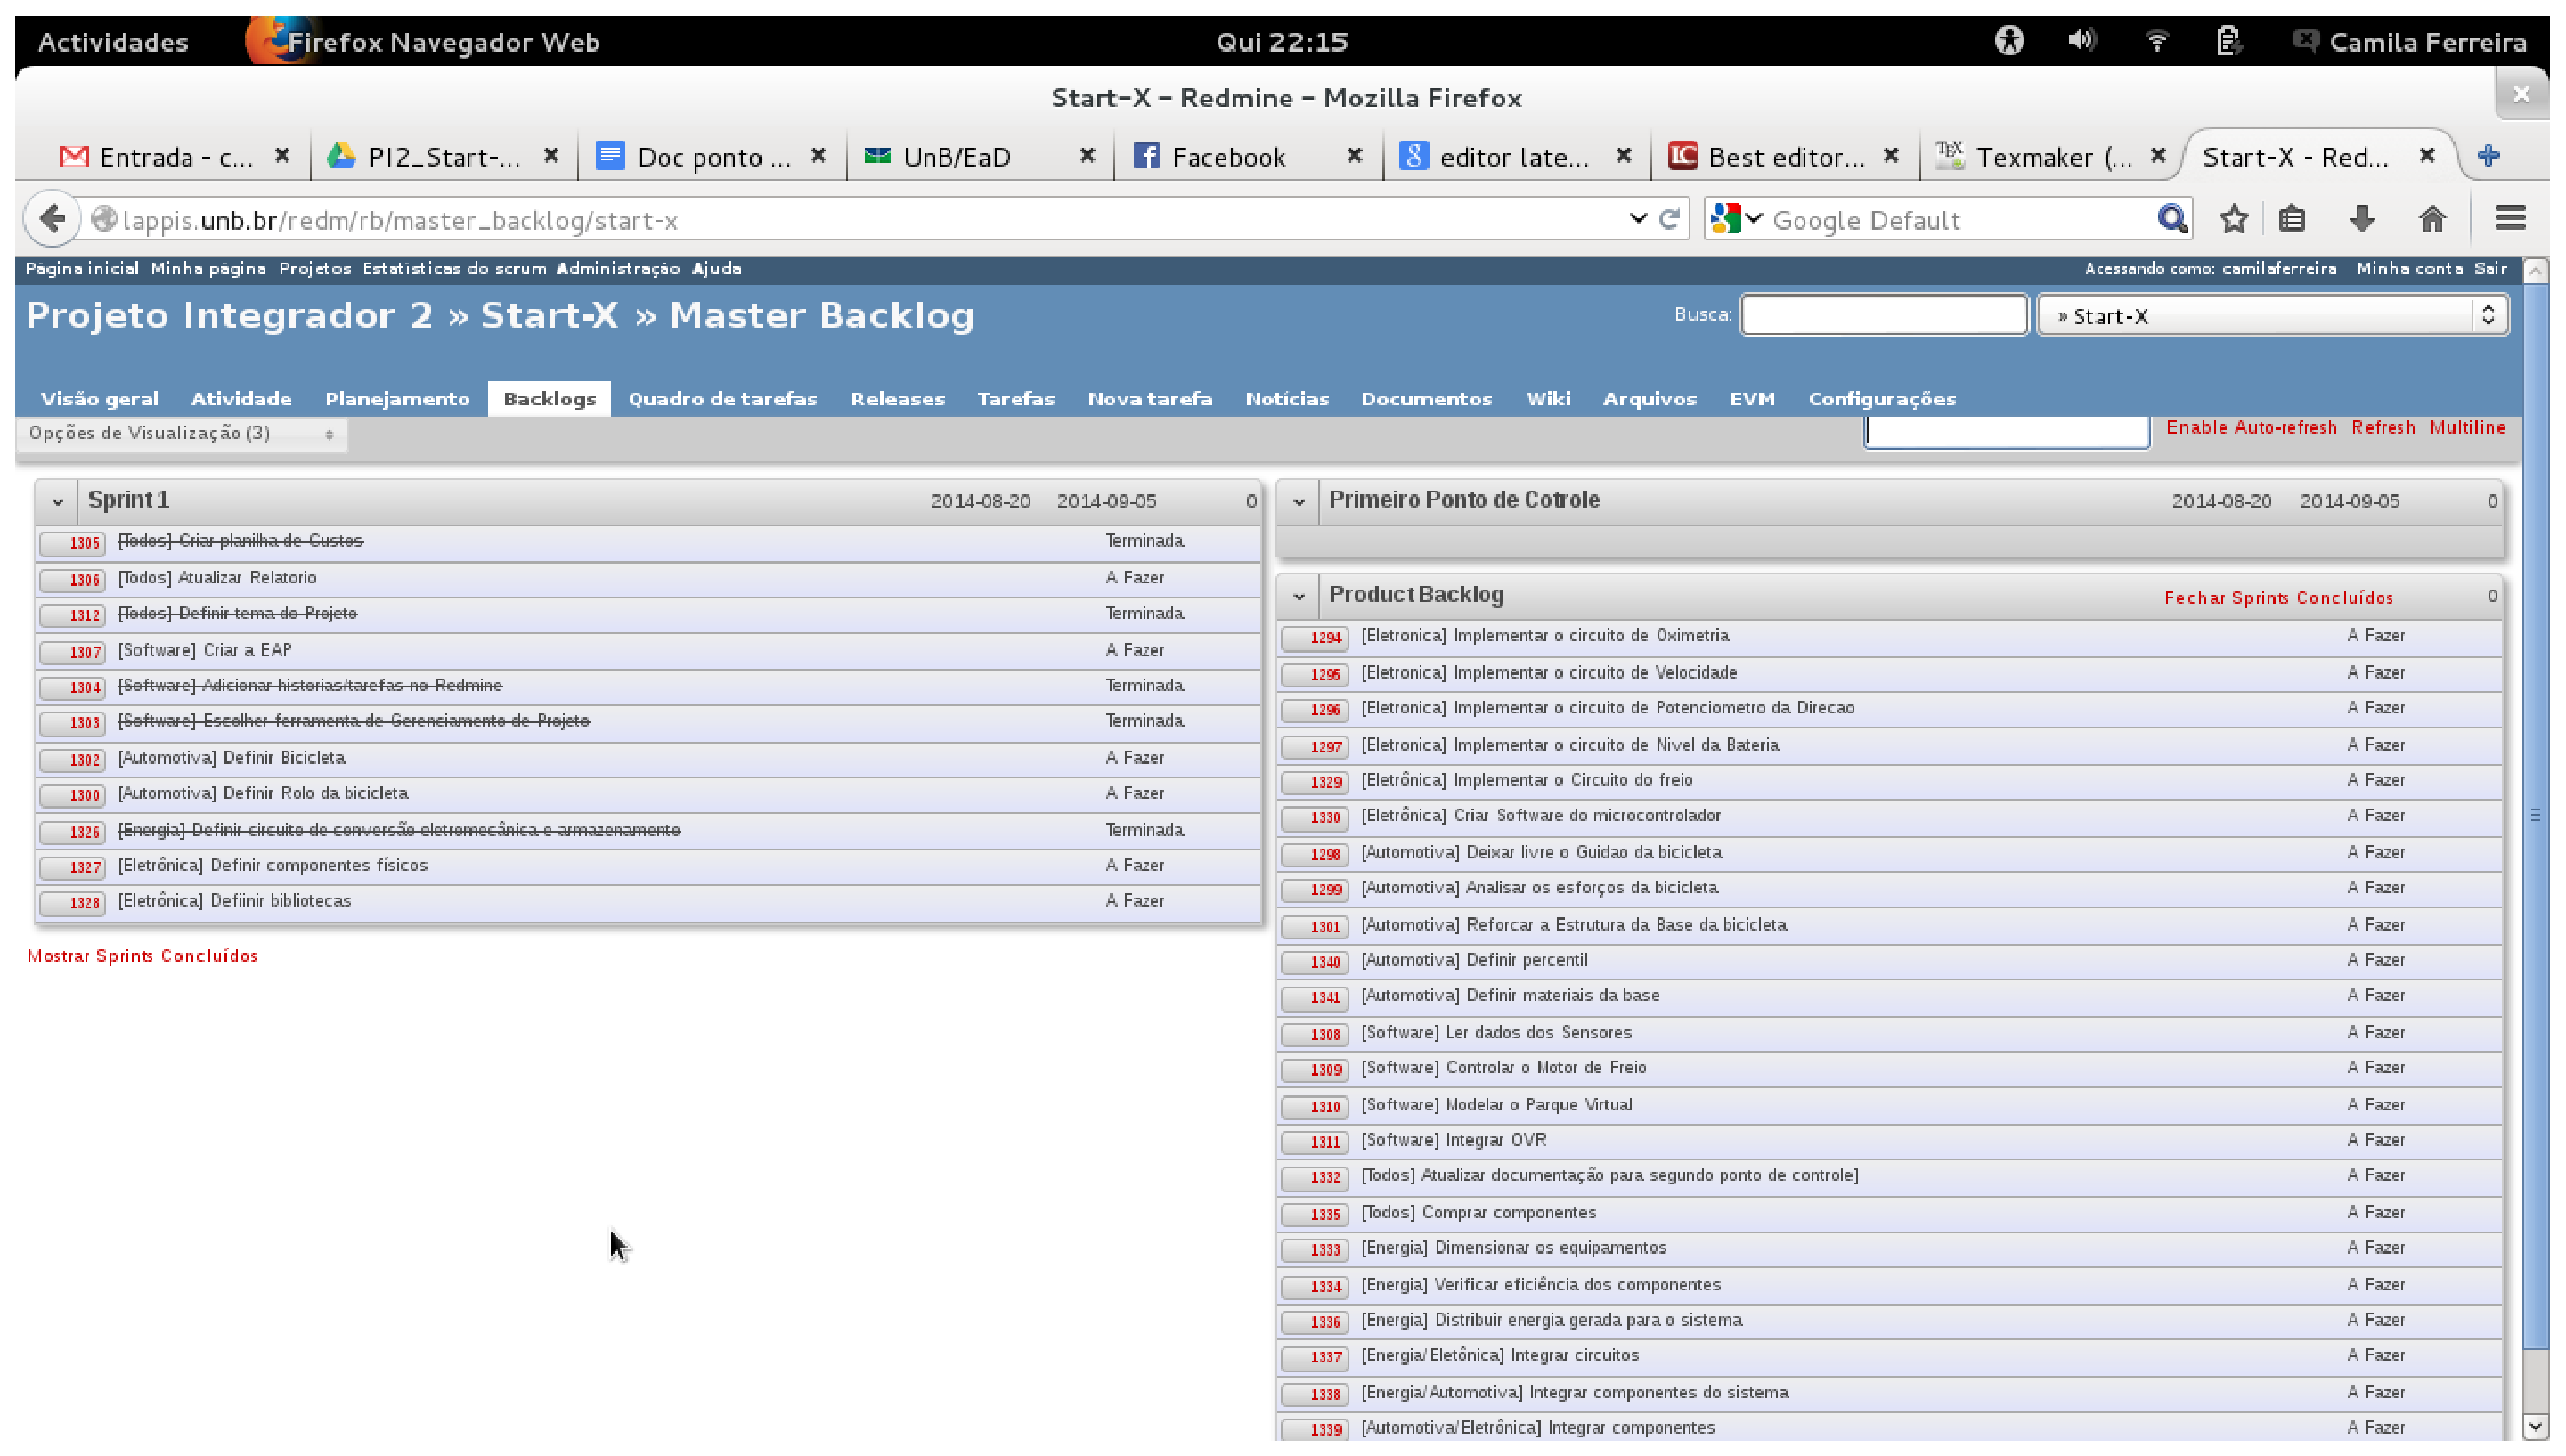
\includegraphics[width=0.8\textwidth]
      {figuras/backlogs.eps}
  \caption[redmine-backlog]
  \label{Redmine e backlog do projeto}
\end{figure}

Para gerir o projeto dividimos o projeto em 3 grandes releases que correspondem com os 3 pontos de controle que teremos duante o semestre. A primeira release se iniciou no primeiro dia de aula de Projeto Integrador 2 e termina no dia do primeiro ponto de controle; a segunda release se iniciará logo após a data do segundo ponto de controle e e terminará no dia do segundo ponto de controle e a terceira relase se iniciará logo após o segundo ponto de controle terminando no dia da entrega final do produto.

\begin{figure}[h]
  \centering
  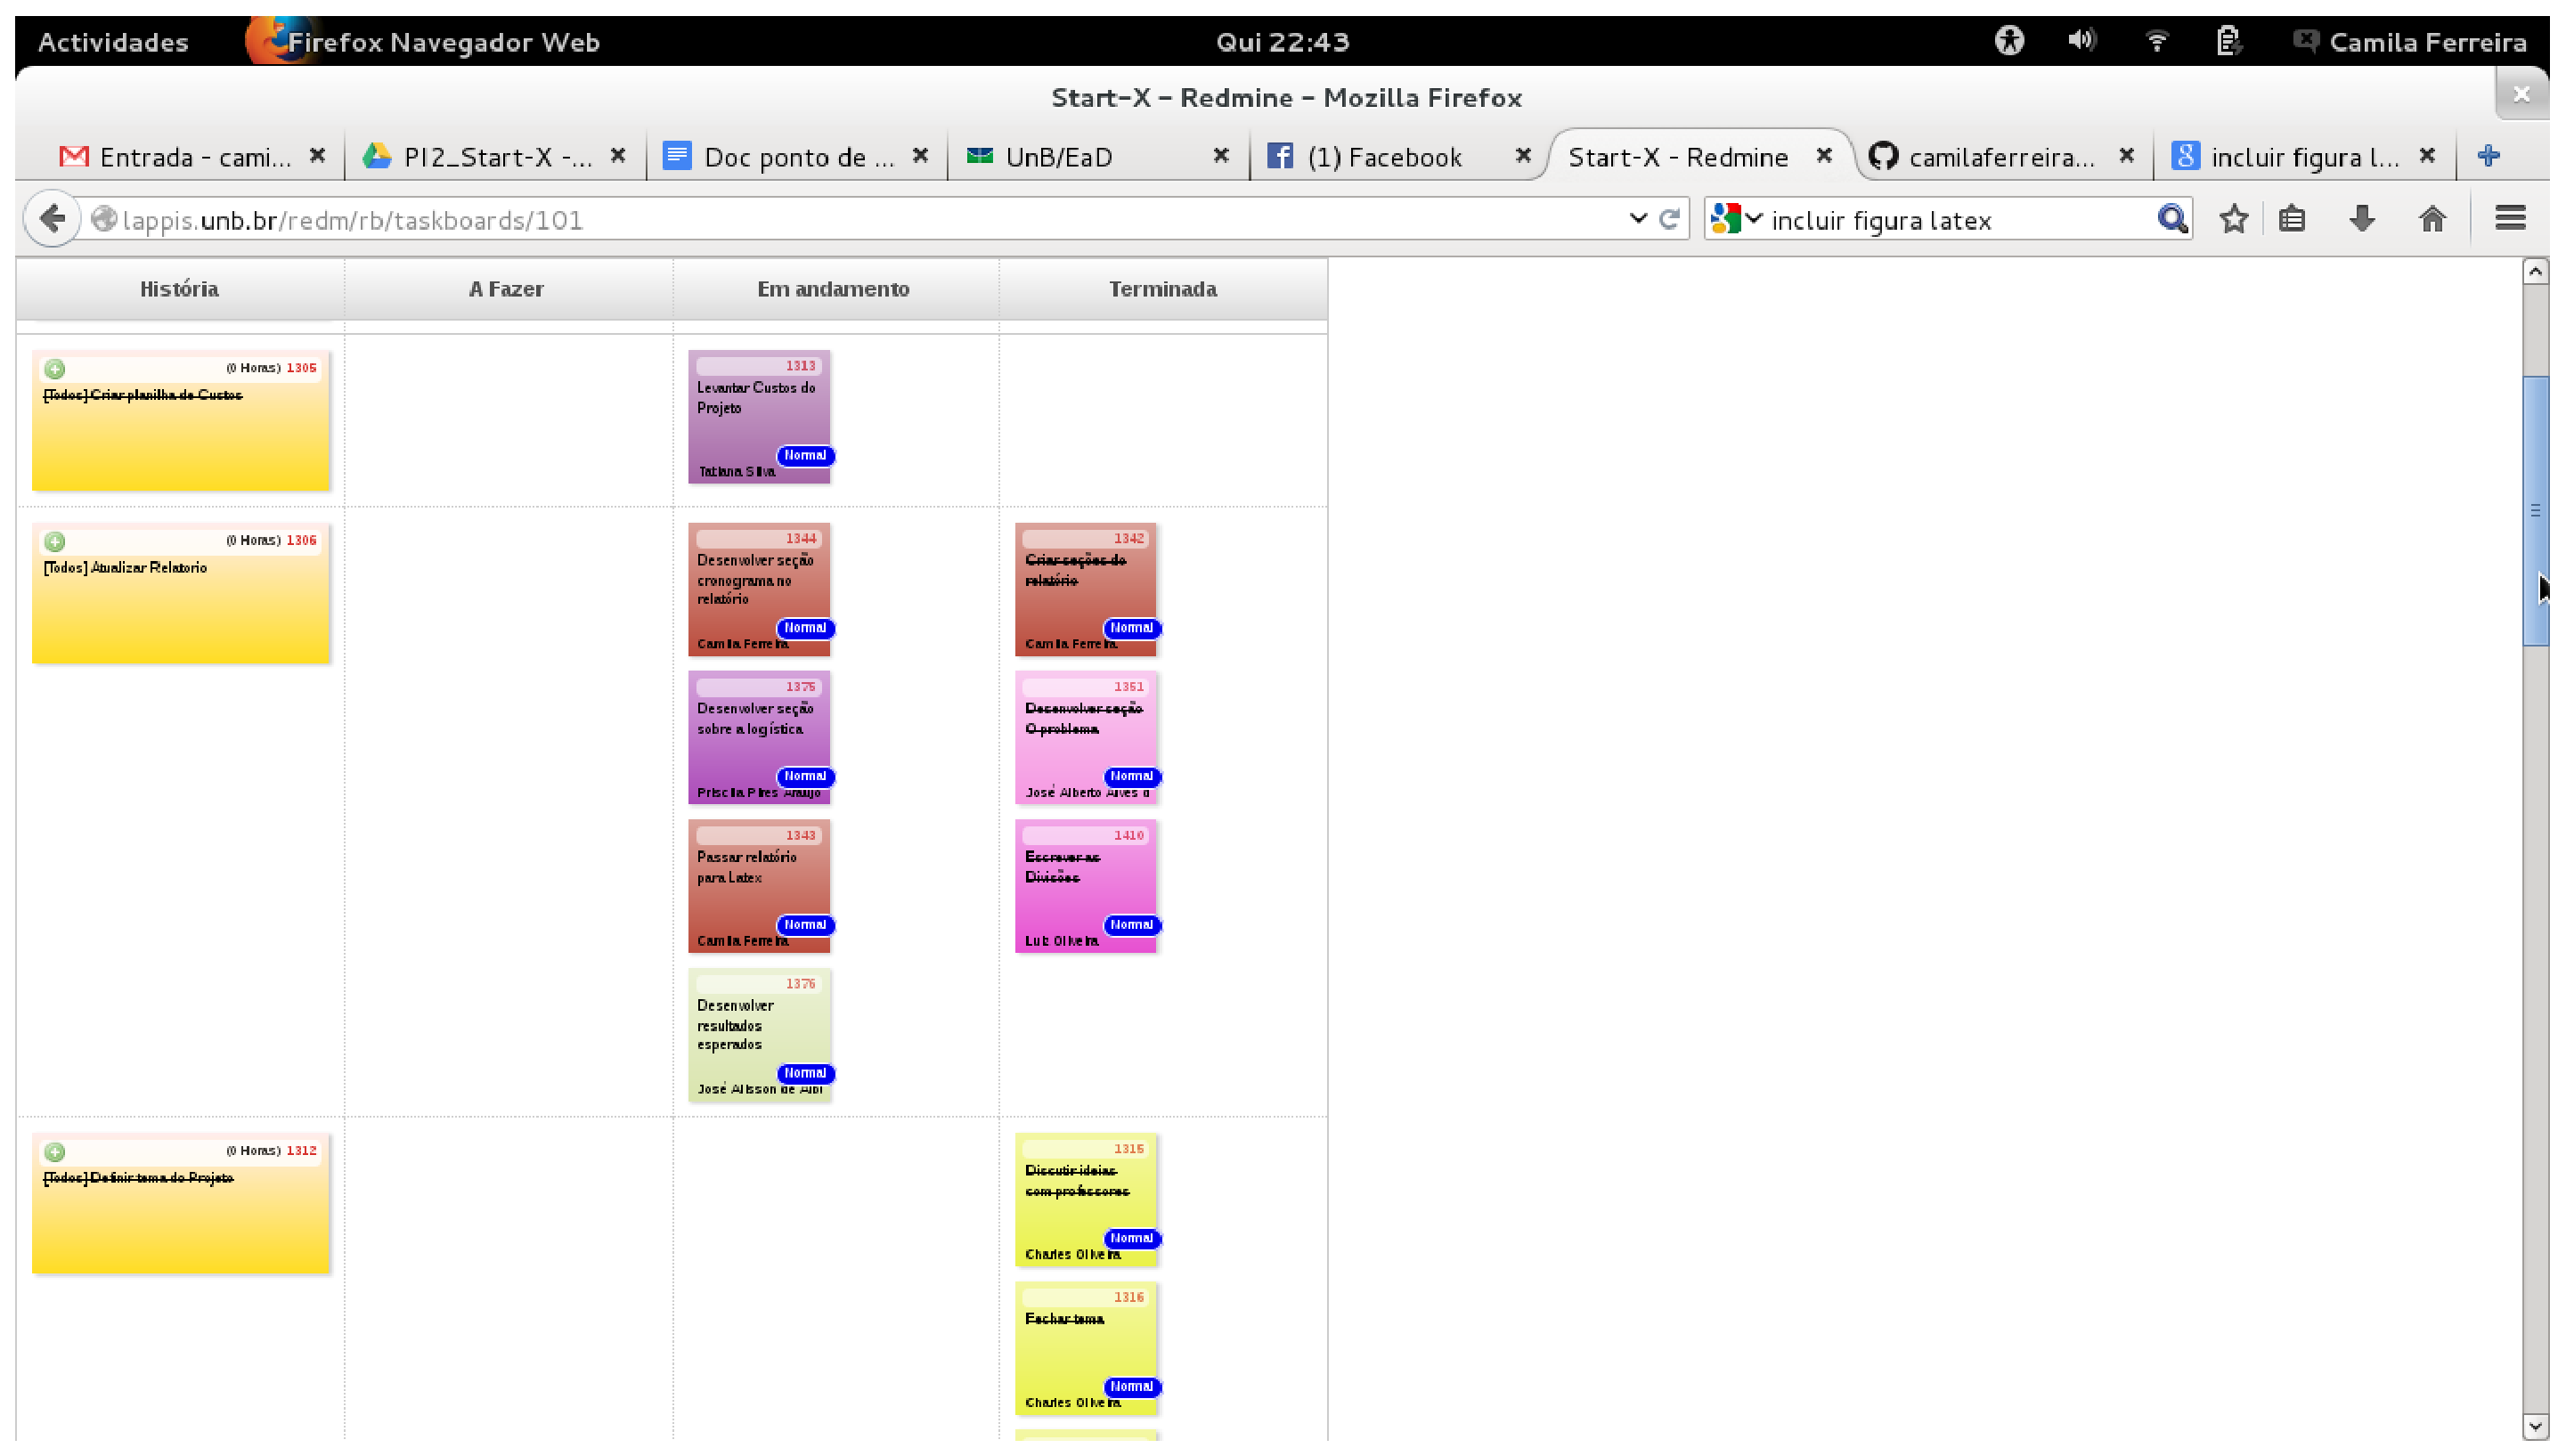
\includegraphics[width=0.8\textwidth]
      {figuras/quadrotarefas.eps}
  \caption[quadro-de-tarefas]
  \label{Quadro de tarefas}
\end{figure}
Para organizar as tarefas do projeto criamos histórias que são macrotarefas onde são posteriormente quebradas em tarefas menores. Essas tarefas são colocadas em um quadro de tarefas.


  

\chapter[Metas]{Metas}

Foram definidas 3 metas para o projeto:

\begin{itemize}
\item Definição do Projeto:
\begin{itemize}
	\item Definição do projeto e entrega do escopo.
\end{itemize}
\item Módulos funcionando separadamente:
\begin{itemize}
	\item  Os módulos do produto devem estar funcionando separadamente.
\end{itemize}
\item Produto concluído
\begin{itemize}
	\item A entrega do produto final com todos os módulos integrados e funcionais.
\end{itemize}
\end{itemize}

\chapter[Financeiro]{Financeiro}
Foi feita estimativa dos custos do projeto em termos de recursos materiais. Os custos relativos à recursos humanos serão calculados e apresentados nos próximos relatórios.

\begin{table}[htbp]
\resizebox{\columnwidth}{!}{%
\begin{tabular}{|p{2.5cm}|p{4.5cm}|p{4.5cm}|p{2.5cm}|p{4.5cm}|}
\hline
\multicolumn{ 5}{|c|}{\textbf{Tabela de custos do projeto}} \\ \hline\hline
\multicolumn{1}{|p{2.5cm}|}{\textbf{Áreas}} & \multicolumn{1}{p{5cm}|}{\textbf{Descrição das etapas}} & \multicolumn{1}{p{4.5cm}|}{\textbf{Materiais}} & \multicolumn{1}{p{2.5cm}|}{\textbf{Quantidade}} & \textbf{Valores} \\ \hline \hline
\multicolumn{ 1}{|p{2.5cm}|}{\textbf{Engenharia Automotiva}} & \multicolumn{ 1}{p{5cm}|}{Compra da bicicleta, após definição do usário} & \multicolumn{ 1}{p{4.5cm}|}{Bicicleta} & \multicolumn{ 1}{p{4.5cm}|}{1 unidade} & \multicolumn{ 1}{p{4.5cm}|}{R\$140.00} \\ 
\multicolumn{ 1}{ |p{2.5cm}|}{} & \multicolumn{ 1}{p{5cm}|}{} & \multicolumn{ 1}{p{4.5cm}|}{} & \multicolumn{ 1}{p{4.5cm}|}{} & \multicolumn{ 1}{p{4.5cm}|}{} \\ \cline{ 2- 5}
\multicolumn{ 1}{ |p{2.5cm}|}{} & \multicolumn{ 1}{p{5cm}|}{Construção do suporte para bicicleta} & Barra de aço chato 1020 & \multicolumn{1}{p{4.5cm}|}{2 metros} & R\$24.00 \\ \cline{ 3- 5}
\multicolumn{ 1}{ |p{2.5cm}|}{} & \multicolumn{ 1}{p{5cm}|}{} & Barra de aço retang. 1020 & \multicolumn{1}{p{4.5cm}|}{2 metros} & R\$30.00 \\ \cline{ 3- 5}
\multicolumn{ 1}{ |p{2.5cm}|}{} & \multicolumn{ 1}{p{5cm}|}{} & Barra de aço circular 1020 & \multicolumn{1}{p{4.5cm}|}{1 metros} & R\$14.00 \\ \cline{ 3- 5}
\multicolumn{ 1}{ |p{2.5cm}|}{} & \multicolumn{ 1}{p{5cm}|}{} & Rolamento de alumínio (rolo) & \multicolumn{1}{p{4.5cm}|}{1 unidade} & R\$70.00 \\ \cline{ 2- 5}
\multicolumn{ 1}{ |p{2.5cm}|}{} & \multicolumn{ 1}{p{5cm}|}{Peças para encaixe da roda traseira} & Conjunto de parafusos/rosca/porcas & \multicolumn{1}{p{4.5cm}|}{x} & R\$40.00 \\ \cline{ 3- 5}
\multicolumn{ 1}{ |p{2.5cm}|}{} & \multicolumn{ 1}{p{5cm}|}{} & Manípulo de Aperto Amaciador & \multicolumn{1}{p{4.5cm}|}{2 unidades} & R\$10.00 \\ \cline{ 3- 5}
\multicolumn{ 1}{ |p{2.5cm}|}{} & \multicolumn{ 1}{p{5cm}|}{} & Borracha para fixação & \multicolumn{1}{p{4.5cm}|}{4 unidades} & R\$30.00 \\ \cline{ 2- 5}
\multicolumn{ 1}{ |p{2.5cm}|}{} & \multicolumn{1}{p{5cm}|}{Junção das barras para o suporte} & Soldagem & \multicolumn{1}{p{4.5cm}|}{x} & R\$60.00 \\ \hline
\textbf{} &  &  &  &  \\ \hline
 & \textbf{Subtotal} & \textbf{} & \textbf{} & \textbf{R\$418.00} \\ \hline
 % &  &  &  &  \\ \hline
 &  &  &  &  \\ \hline\hline
\multicolumn{ 1}{|p{2.5cm}|}{\textbf{Engenharia Eletrônica}} & \multicolumn{ 1}{p{5cm}|}{Leitura da velocidade do ciclista} & Circuito & \multicolumn{1}{p{4.5cm}|}{1 unidade} & R\$3.00 \\ \cline{ 3- 5}
\multicolumn{ 1}{ |p{2.5cm}|}{} & \multicolumn{ 1}{p{5cm}|}{} & Sensor de velocidade & \multicolumn{1}{p{4.5cm}|}{1 unidade} & R\$170.00 \\ \cline{ 2- 5}
\multicolumn{ 1}{ |p{2.5cm}|}{} & \multicolumn{ 1}{p{5cm}|}{Leitura dos batimentos cardíacos do ciclista} & Circuito & \multicolumn{1}{p{4.5cm}|}{1 unidade} & R\$3.00 \\ \cline{ 3- 5}
\multicolumn{ 1}{ |p{2.5cm}|}{} & \multicolumn{ 1}{p{5cm}|}{} & Sensor de oximetria & \multicolumn{1}{p{4.5cm}|}{1 unidade} & R\$10.00 \\ \cline{ 2- 5}
\multicolumn{ 1}{ |p{2.5cm}|}{} & \multicolumn{1}{p{5cm}|}{Leitura do nível da bateria} & Sensor de nível de bateria & \multicolumn{1}{p{4.5cm}|}{1 unidade} & R\$10.00 \\ \cline{ 2- 5}
\multicolumn{ 1}{ |p{2.5cm}|}{} & \multicolumn{1}{p{5cm}|}{Medir o giro do guidão} & Potenciômetro p/ guidão & \multicolumn{1}{p{4.5cm}|}{1 unidade} & R\$1.00 \\ \cline{ 2- 5}
\multicolumn{ 1}{ |p{2.5cm}|}{} & \multicolumn{1}{p{5cm}|}{Leitor dos sensores} & 1 micro msp 430 & \multicolumn{1}{p{4.5cm}|}{1 unidade} & R\$30.00 \\ \cline{ 2- 5}
\multicolumn{ 1}{ |p{2.5cm}|}{} & \multicolumn{1}{p{5cm}|}{Frenar a bicicleta} & Servo motor & \multicolumn{1}{p{4.5cm}|}{1 unidade} & R\$40.00 \\ \cline{ 2- 5}
\multicolumn{ 1}{ |p{2.5cm}|}{} & \multicolumn{1}{p{5cm}|}{Ventilação do ciclista} & Cooler & \multicolumn{1}{p{4.5cm}|}{2 unidade} & R\$100.00 \\ \hline
 &  &  &  &  \\ \hline
 & \textbf{Subtotal} &  &  & \textbf{R\$367.00} \\ \hline
 % &  &  &  &  \\ \hline
 &  &  &  &  \\ \hline \hline
\multicolumn{ 1}{|p{2.5cm}|}{\textbf{Engenharia de Energia}} & \multicolumn{1}{p{5cm}|}{Transforma energia mecânica em elétrica} & Alternador & \multicolumn{1}{p{4.5cm}|}{1 unidade} & R\$230.00 \\ \cline{ 2- 5}
\multicolumn{ 1}{ |p{2.5cm}|}{} & \multicolumn{1}{p{5cm}|}{Armazenamento de energia} & No break (bateria, tomadas e inversor) & \multicolumn{1}{p{4.5cm}|}{1 unidade} & R\$260.00 \\ \cline{ 2- 5}
\multicolumn{ 1}{ |p{2.5cm}|}{} & \multicolumn{1}{p{5cm}|}{Medição} & Multímetro & \multicolumn{1}{p{4.5cm}|}{2 metros} & R\$40.00 \\ \cline{ 2- 5}
\multicolumn{ 1}{ |p{2.5cm}|}{} & \multicolumn{ 1}{p{5cm}|}{Distribuição de energia} & Cabos (chicotes) & \multicolumn{1}{p{4.5cm}|}{1 unidade} & R\$18.00 \\ \cline{ 3- 5}
\multicolumn{ 1}{ |p{2.5cm}|}{} & \multicolumn{ 1}{p{5cm}|}{} & Cabos tipo jacaré & \multicolumn{1}{p{4.5cm}|}{4 unidade} & R\$16.00 \\ \hline
 &  &  &  &  \\ \hline
 & \textbf{Subtotal} &  &  & \textbf{R\$564.00} \\ \hline
 % &  &  &  &  \\ \hline
 &  &  &  &  \\ \hline \hline
\multicolumn{ 1}{|p{2.5cm}|}{\textbf{Engenharia de Software}} & \multicolumn{ 1}{p{5cm}|}{Óculos usado para simular ambiente virtual} & \multicolumn{ 1}{p{4.5cm}|}{Oculus Rift} & \multicolumn{ 1}{p{4.5cm}|}{1 undiade} & \multicolumn{ 1}{p{4.5cm}|}{R\$1,500.00} \\ 
\multicolumn{ 1}{ |p{2.5cm}|}{} & \multicolumn{ 1}{p{5cm}|}{} & \multicolumn{ 1}{p{4.5cm}|}{} & \multicolumn{ 1}{p{4.5cm}|}{} & \multicolumn{ 1}{p{4.5cm}|}{} \\ \hline
 &  &  &  &  \\ \hline
 & \textbf{Subtotal} &  &  & \textbf{R\$1,500.00} \\ \hline
 % &  &  &  &  \\ \hline
 &  &  &  &  \\ \hline \hline
 & \textbf{Total} &  &  & \textbf{R\$2,849.00} \\ \hline
\end{tabular}
}
\caption{Planilha de custos com equipamentos/materiais}
\label{fabela_fudida}
\end{table}

Considerando o valor médio ganho por um estagiário de Engenharia como 900,00 reais,
com 20 horas semanais temos que uma hora de um estagiário de engenharia equivale a
11,25 reais.

Consideramos 6 horas de trabalho por semana em 16 semanas dedicadas ao projeto Start-X.

\begin{table}[h]
\centering
\begin{tabular}{|l|c|l|}
\hline
Integrante       & \multicolumn{1}{l|}{Horas Trabalhadas} & Valor Total \\ \hline
Camila Ferreira  & 96                                     & R\$1,080     \\ \hline
Charles Daniel   & 96                                     & R\$1,080     \\ \hline
Gabriela Navarro & 96                                     & R\$1,080     \\ \hline
José ALberto     & 96                                     & R\$1,080     \\ \hline
José Alisson     & 96                                     & R\$1,080     \\ \hline
Júlio Cezar      & 96                                     & R\$1,080     \\ \hline
Lucas Kanashiro  & 96                                     & R\$1,080     \\ \hline
Luiz Fernando    & 96                                     & R\$1,080     \\ \hline
Macarcur Sousa   & 96                                     & R\$1,080     \\ \hline
Priscila Pires   & 96                                     & R\$1,080     \\ \hline
Tatiana Dias     & 96                                     & R\$1,080     \\ \hline
Thiago Ferreira  & 96                                     & R\$1,080     \\ \hline
\multicolumn{2}{|r|}{Total}                               & R\$12,960    \\ \hline
\end{tabular}
\caption{Planilha de custos com pessoal.}
\end{table}

Custo Total

\begin{table}[h]
\centering
\begin{tabular}{|l|l|}
\hline
Tipos de custo              & Valor       \\ \hline
Equipamentos/materiais      & R\$2,849.00 \\ \hline
Pessoal                     & R\$12,960   \\ \hline
\multicolumn{1}{|r|}{Total} & R\$15,809   \\ \hline
\end{tabular}
\caption{Custo total do projeto}
\end{table}


 
 

\part{Conclusões}
\chapter[Resultados]{Resultados}

Com a inclusão dos sensores no sistema, espera-se coletar dados que são considerados importantes para as mudanças físicas que irão ocorrer no ambiente virtual, bem como causar sensações no usuário de forma que o mesmo tenha um experiência semelhante a andar de bicicleta na rua. Os seguintes dados serão coletados: velocidade, direção a qual o guidão é movimentado e nível da bateria para o sistema de realimentação.

Os dados da velocidade serão apresentados ao atleta para que ele tenha consciência do seu desempenho. O sinal do sensor de direção do guidão fará com que haja uma alteração no ambiente virtual, ou seja, dependendo da angulação do guidão, o usuário terá a sensação de que está fazendo uma curva. Outro dado importante é que quando houver uma subida no percurso do ambiente virtual o usuário terá maior dificuldade ao pedalar, como se realmente estivesse subindo um morro, por exemplo.

Por meio destas características, espera-se simular um ambiente que seja tão próximo quanto possível da realidade de forma a tornar atividades físicas, como o \textit{spinning}, algo menos monótono já que o atleta não se desloca e apresentar dados que possam melhorar seu rendimento. Outro resultado interessante é realizar a comparação do nível de iteratividade do sistema com uma situação real e analisar como o usuário se comporta em ambos os ambientes. Isso é interessante para atletas de alto nível pois simular o percurso de uma prova e ter conhecimento das reações do corpo naquele ambiente é de fundamental importância para um bom desempenho.

\chapter{Manual do Produto} % (fold)
\label{cha:manual_do_produto}
 
O trecho a seguir descreve o processo recomendado pela equipe para o uso do produto, assim como os cuidados que devem ser tomados com o manuseio.

\section{Modo de Uso} % (fold)
\label{sec:modo_de_uso}

\begin{enumerate}
	\item Verifique se a aplicação já esta em funcionamento com o auxilio da tela secundaria (notebook/monitor).
	\item Posicione-se sobre a bicicleta. Verifique se a mesma se mantem  estável com o seu peso. Para mais informações sobre os valores para qual este produto foi projetado, verificar \autoref{dados-usuario}.
	\item Imerja-se na realidade virtual com o \gls{rift}.
	\item Após o uso do equipamento, remova o \gls{rift} e espere de 15 a 30 segundos antes de tentar desmontar da bicicleta\footnote{Devido a alta imersão, é recomendado um tempo para se acostumar novamente com a realidade antes de realizar movimentos bruscos.}.
\end{enumerate}

\section{Precauções} % (fold)
\label{sec:precau_es}

\begin{description}
	\item [Não tente desmontar da bicicleta utilizando o gls{rift}] $-$ Ao utilizar o \gls{rift}, a imersão proporcionará uma perca da noção de espaço e posição da realidade. Tentar se movimentar na realidade visualizando o ambiente virtual é extremamente desencorajador.
	\item [Não grite] $-$ A imersão no ambiente virtual causa uma perca de contato com a realidade, lembre-se disto antes de tentar se comunicar com aqueles que te assistem.
	\item [Evite balançar muito na bicicleta ou ficar em pé nela] $-$ Apesar de cálculos terem sido feitos no intuito de manter a bicicleta o mais estável possível ao chão, o produto ainda é passível de tombamento quando exposto a determinados momentos angulares.
	\item [Divirta-se] $-$ Mesmo tendo como objetivo apresentar uma alternativa para a pratica de atividades físicas em ambientes fechados, o projeto busca oferecer também entretenimento ao usuário.
	\item [Mantenha o produto] $-$ Evite reajustar os sensores, a altura do guidão ou do banco. Por ser um protótipo, o produto ainda não oferece um amplo grau de personalização. Tentar configurar o equipamento sem o devido conhecimento do produto pode vir a danifica-lo ou  ao comprometimento dos sinais adquiridos para controle do ambiente.
\end{description}

\bookmarksetup{startatroot} 

\postextual

\bibliography{bibliografia} 

\printindex

\glsaddall
\part*{Gloss\'ario}
\providetranslation{Notation (glossaries)}{Notação}
\providetranslation{Description (glossaries)}{Descrição}
\phantomsection
\addcontentsline{toc}{part}{Gloss\'ario}
\glossarystyle{altlisthypergroup}
\printglossary[title= ]

% \newpage
% \phantomsection
% \addcontentsline{toc}{chapter}{Lista de Termos}\label{acrom}
% \printglossary[type=\acronymtype,title=Lista de Termos,toctitle=Lista de Termos]


\end{document}

